\section{Graphical Editor}\label{sec:intocps}

Currently, several external tools are required for the creation and composition of co-simulation scenarios.
The primary goal of the development of an integrated graphical editor is to integrate the functionality of these tools and provide a more efficient work-flow.
We refer to this editor as the \emph{Graphical Editor}.

The editor aims to provide an interaction that is familiar to users of modelling software such as 20-sim, OMEdit or Simulink.
Common for these is that they provide a block-based design flow which allows the user to compose scenarios by dragging components from a library onto a canvas.
The scenarios are further elaborated by dragging connections between compatible ports. 

An outline of the editor and its different panels can be seen in Figure~\ref{fig:scenario_editor_overview}.
%As seen on the figure the editor is split into multiple panels.
The functionality of each of these is described in the subsections below.


\begin{figure}[bt]



\makebox[\textwidth]{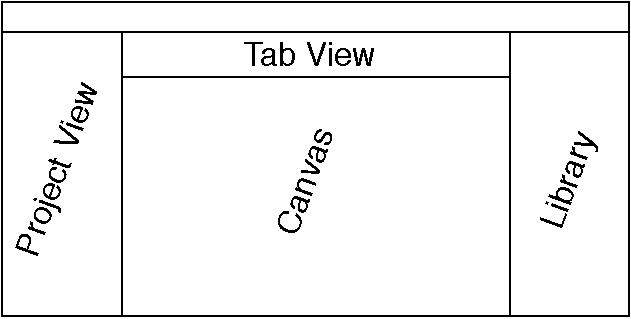
\includegraphics[width=1\columnwidth]{Images/scenario_editor_overview.pdf}}
\caption{Mock-up of the envisioned editor annotated with the names of its constituent parts.}
\label{fig:scenario_editor_overview}
\end{figure}



\subsection{Project View}
The \emph{project view} provides a tree view of the current project's \emph{artefacts}.
An example of these, and the relation between project view and the canvas are is depicted in Figure~\ref{fig:project_view}.
As shown these are categorised based on their type such as components and connections.
Artefacts may themselves be hierarchically composed as is the case of the "cont" component.
In these cases they may be expanded in the tree to reveal their internal contents.

\begin{figure}[bt]
\makebox[\textwidth]{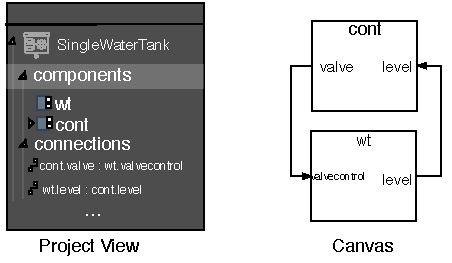
\includegraphics[width=0.7\columnwidth]{Images/project_view.pdf}}
\caption{Project view and canvas relationship}
\label{fig:project_view}
\end{figure}


%It is important to emphasise that an artefact does not always correspond to some specific file.
%Take for example the artefact \emph{wt} in the components category.
%Its presence is merely stating that an instance of the specific type component the standard WaterTank example %exists at the top level of the hierarchy.
%In the underlying SSP package this information will be stored as an XML element, not a separate file.


\subsection{Composition}
A central part of defining a simulation scenario is defining instances of components and how these are connected. 
Instances are created by dragging an item from the \emph{components-group} into the diagram as seen in figure~\ref{fig:connecting_fmus}.
Naturally every instance must be assigned a name. This may be handled by either prompting the user upon creation or automatically resolving the instance name based on the component name as seen in figure~\ref{fig:connecting_fmus}a.

After having instantiated the needed components the connections between their ports may be established. 
Ports are represented by symbols reminiscent of a less-than sign with the name of the port next to it.
An input is indicated by a symbol pointing inwards whereas an output is indicated by a symbol pointing outwards.
This representation is proposed as it is compact and shows the name and direction of a port.

A pair of ports are connected by hovering the mouse over an unconnected output port, initiating a drag and finally releasing the drag over an unconnected input port.
To limit the probability of connecting ports incorrectly the GUI will not accept a connection from the source port to an incompatible target.
An simple rule is to check if the units of the two ports matches, but it is possible to imagine more elaborate validation procedures.

\begin{figure}[bt]
\centering
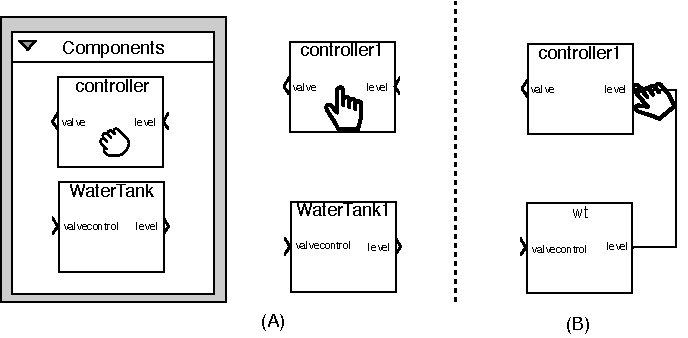
\includegraphics[width=0.8\columnwidth]{Images/connecting_fmus.pdf}
\caption{Illustration depicting how the inputs and outputs of FMUs may be connected graphically.}
\label{fig:connecting_fmus}
\end{figure}



\subsection{Parameterisation}
A component may expose several parameters allowing its behaviour to be adjusted without the need to modify its implementation. This process is referred to as parameterisation.
In the context of the running example a parameter of the water tank component would be its area or the gravitational constant. Double clicking on a component instance will open an \emph{configuration-window}, as seen in figure~\ref{fig:parameterization}. The window contains a section which list all available parameters of the component.
A concrete value may be entered for a given parameter, or it may be bound to a parameter of the parameter set.

\begin{figure}[bt]
\centering
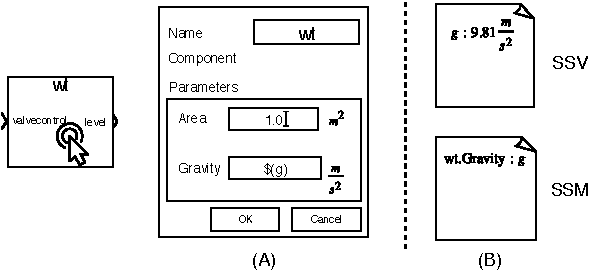
\includegraphics[width=0.8\columnwidth]{Images/parameterization.pdf}
\caption{Parameterization of a component. A \emph{configuration-window} is opened when a component is double clicked.}
\label{fig:parameterization}
\end{figure}



The editor allows such bindings to be defined directly from the configuration-window.
In the context of the editor these are referred to as \emph{parameter-binding}.
The bindings are defined using a special notation: \emph{\$(parameter)}, as seen on \ref{fig:parameterization}a.

The bound parameters of the components now refer to the value of the corresponding parameters of the parameter set.
An example of how this may be used would be if multiple water tanks existed, in this case they would all depend on the gravitational acceleration, $g$, experienced in their environment.
Using the binding mechanism the value of $g$ may adjusted in the parameter set to examine its impact on the whole system's performance.

From a users standpoint it would be useful to know the valid ranges and constraints of a parameter's values. This would allow the editor to inform the user of any inconsistencies during configuration rather than resulting in error during simulation. The SSP standard itself does not define any mechanism for specifying these. However, due to its extensibility it would be possible to implement a layered standard for this purpose.


\subsection{Representing Hierarchy}

A central feature of the SSP standard is its ability to describe hierarchical systems.
Specifically it allows for the composition of a system from multiple subsystems, which may themselves be SSP-packages.

More related to the editor itself is how the hierarchy of components is represented.
20-sim and Simulink both allow the creation and navigation of this hierarchy graphically.
Both use a very similar approach, the primary differences being notation.
An an example of what this may look like in the editor is shown in Figure~\ref{fig:subsystems}.

\begin{figure}[bt]
\centering
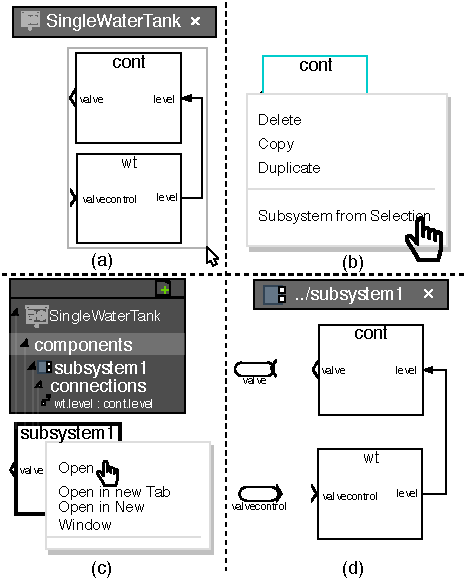
\includegraphics[width=0.7\columnwidth]{Images/subsystems.pdf}
\caption{Proposed method to create subsystem from a selection of components. (a) components are selected. (b) "Subsystem from Selection" is selected in the context menu. (c) the two components have been converted into a single subsystem, which is double clicked to access the internal view. (d) internal view of the subsystem.}
\label{fig:subsystems}
\end{figure}


Navigation is straightforward, double clicking a subsystem changes the view such that it shows the subsystems internals.
We refer to this as \emph{opening} a subsystem.
This process can be repeated to reach deeper into the hierarchy.
Given the lack of a parent component to click on, navigating upwards is done using a toolbar button.

The process of creating subsystems from existing components may be done in the following way.
First one or more components are selected, then the "Subsystem from Selection" item is chosen from the context menu.
This results is a new subsystem in place of the selected components.
The subsystem contains the now replaced components.

\subsection{Semantic Adaptations}\label{ssec:semantic_adaptations}

%While the FMI standard defines a common format for exchanging FMUs it does not guarantee the absence of so called \emph{interaction mismatches} when these are composed \cite{Gomes&18a}.
%The goal of semantic adaptations is to allow these mismatches to be corrected without the need to %involve the original author of the FMU.

A solution is proposed that allows different types of semantic adaptations graphically using the familiar drag and drop system, as shown in Figure~\ref{fig:semantic_adaptations}.
A group containing entries corresponding to commonly used types of adaptations is added to the library.
An adaptation can be dragged onto a component thereby "decorating" it with the adaptation.
The parameters of an adaptation may be configured in a similar fashion to how a component is parameterised.

The suitability of this approach relies on the available adaptations being sufficiently modular, such that they can be composed to cover most needs.
Alternatively, its possible to imagine an "DSL"-adaptation which allows for arbitrary adaptations made in a domain specific language.



\begin{figure}[bt]
\centering
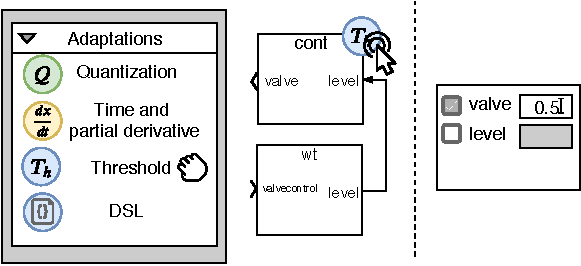
\includegraphics[width=0.9\columnwidth]{Images/semantic_adaptation.pdf}
\caption{applying and configuring of semantic adaptations.}
\label{fig:semantic_adaptations}
\end{figure}

